\section{Development process}

The development part of this exercise was, as with the previous ones, done at the computer lab in the IT-Vest building at NTNU (room ITV-458). The lab is equipped with workstations connected to the EFM32GG-DK3750 development board made by Energy Micro.
The subject staff provided us with a framework on which to base our work, more on this in section \ref{project-setup-toolchain}.
As per usual, we put the project under version control immediately to ease collaboration. Seeing as this is a multipart exercise, collaboration aided by version control became an important aspect of the process to a larger degree than in the previous exercises.
\subsection{Devices}
The device used in this exercise is the same as in the previous exercise, the EFM32GG-DK3570 produced by Silicon Labs. It has a built in Digital-Analog Converter which is the primary focus of the exercise.

While the DAC is physically connected to the main processing unit, it functions like a peripheral that must be manually activated before it can be used. A standard $3.5mm$ audio jack socket is available, meaning a normal set of headphones or earplugs can be connected to listen to the DAC output.

As in exercise 1 the only source of user input is the 8-button gamepad peripheral connected to the development board's GPIO pins. In this exercise the 8 LEDs on the gamepad are not the primary means of output, but they are still available if needed.

\begin{figure}[h!]
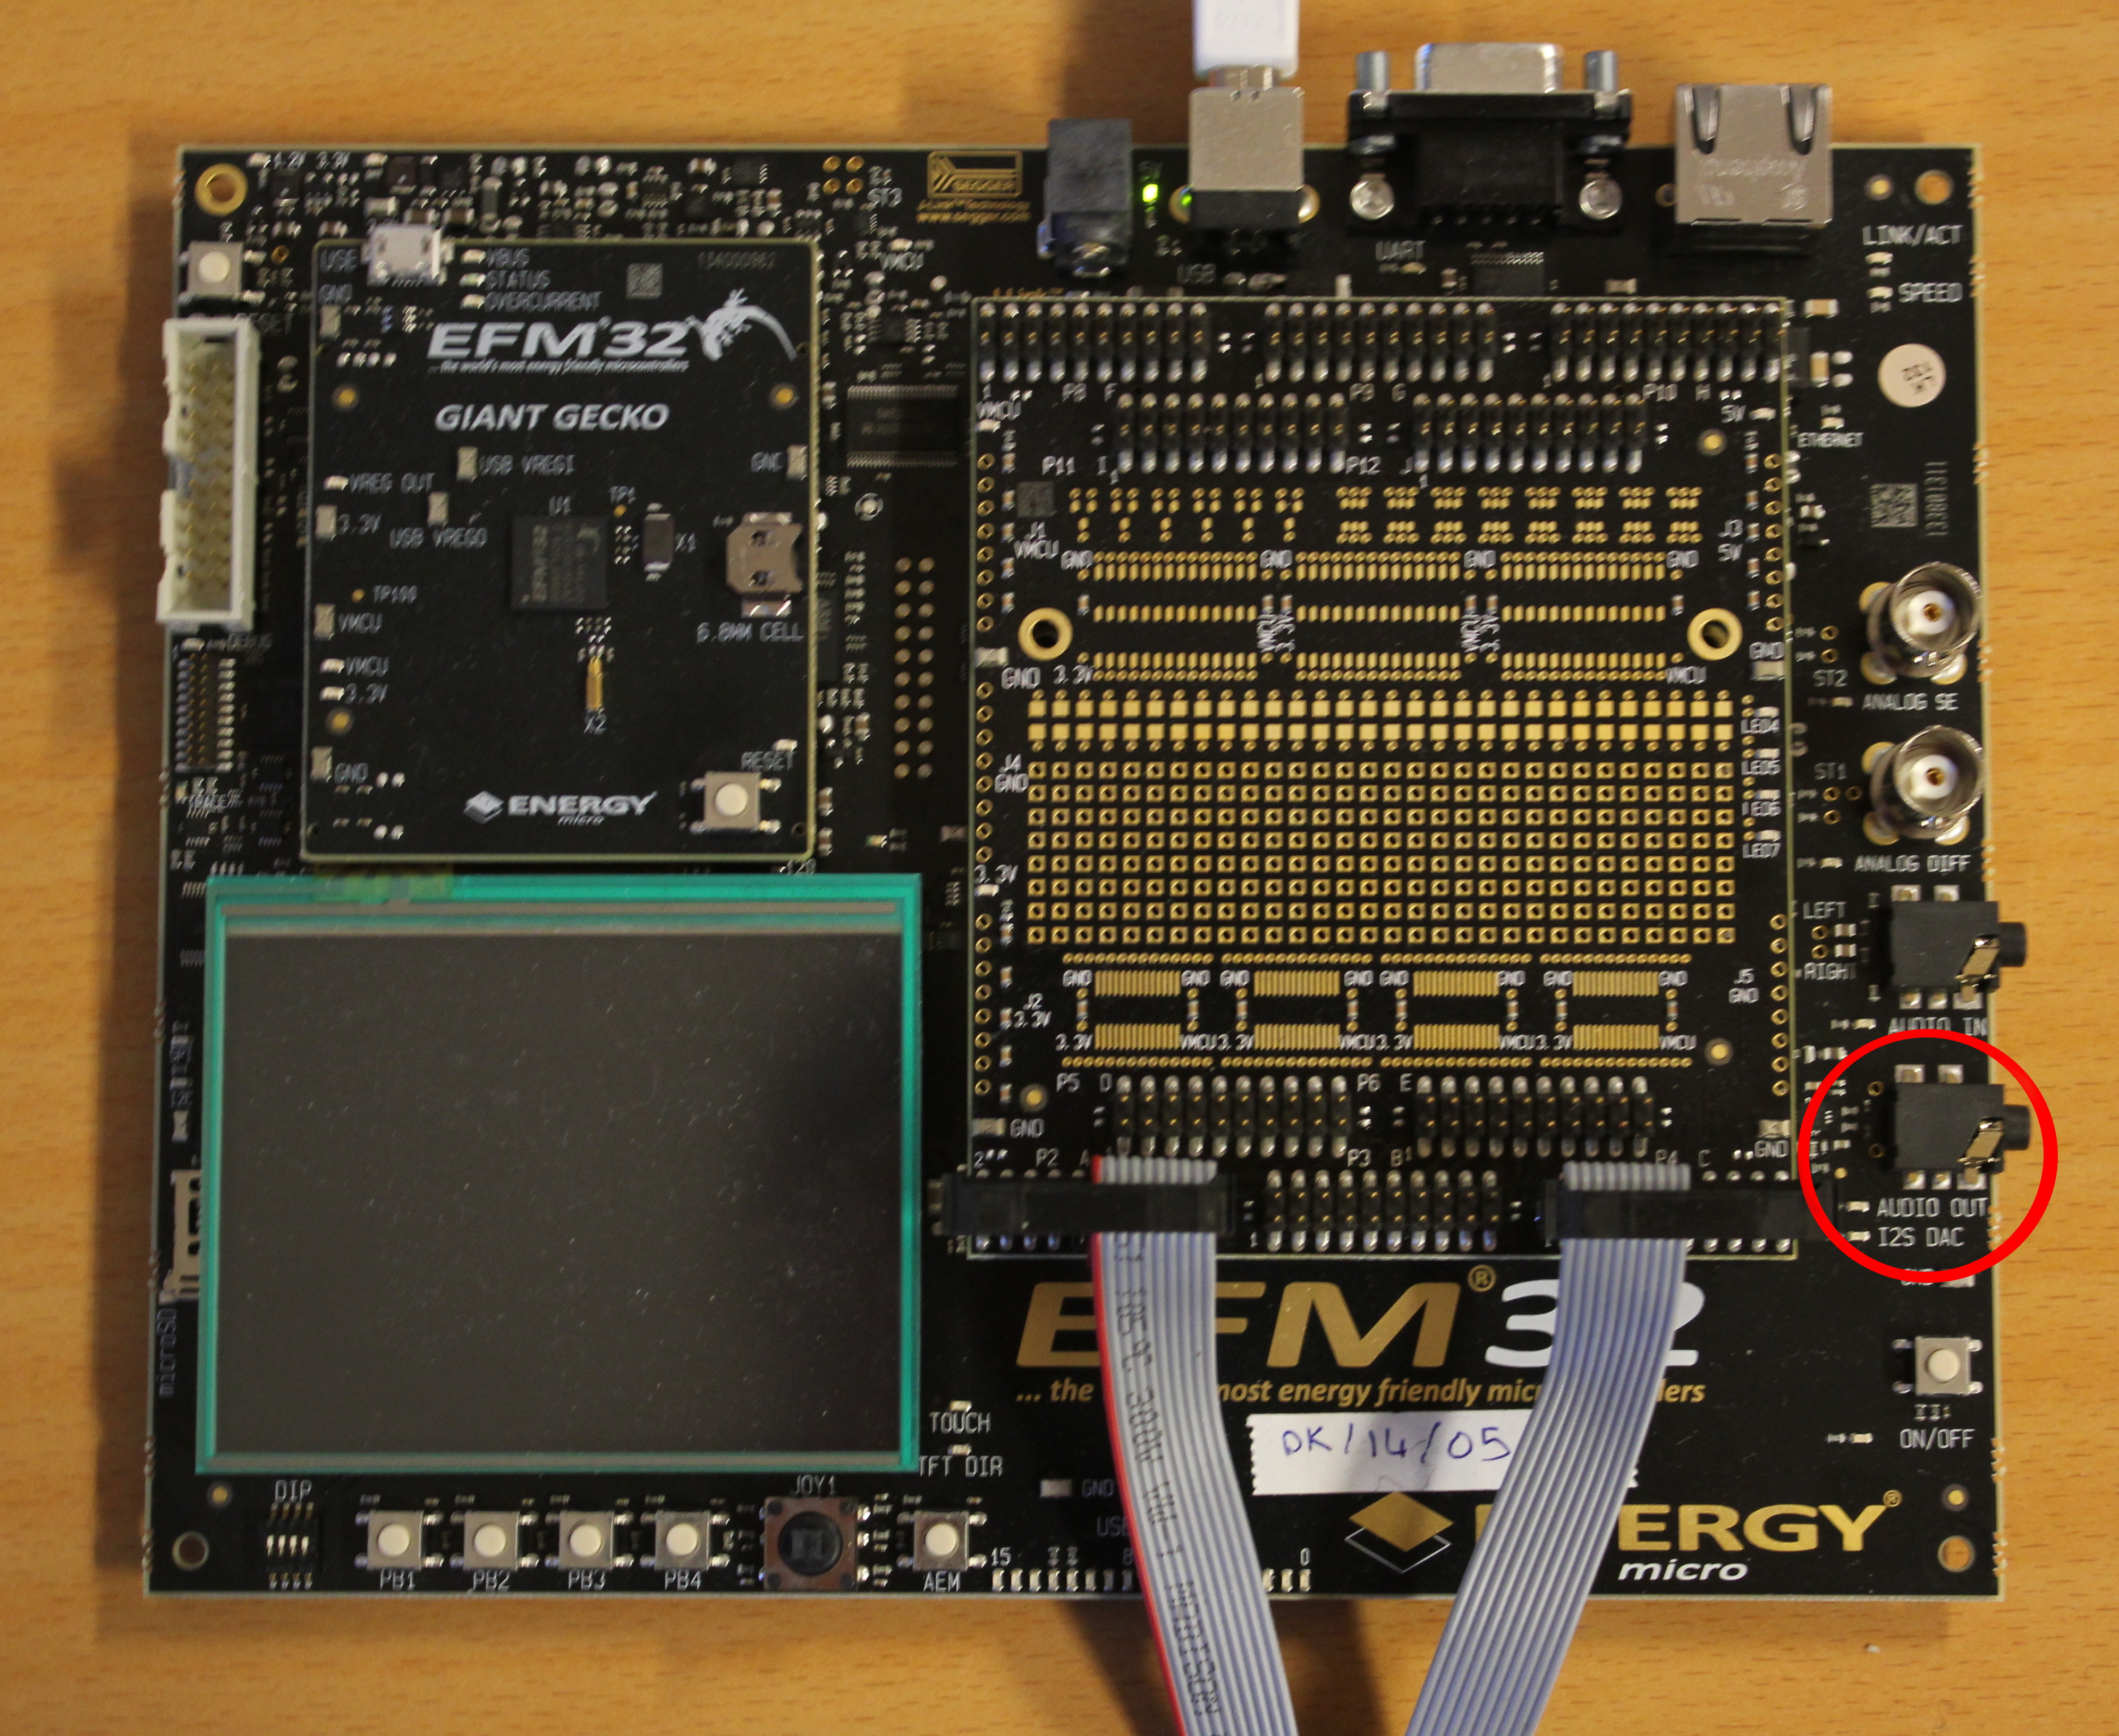
\includegraphics[width=\linewidth]{img/efm32gg.JPG}
\caption{The EFM32GG-DK3570. Highlighted with red is the audio output from the DAC. The gamepad peripheral is connected by the cables emerging on the bottom of the picture.}
\label{fig:efm32gg}
\end{figure}

